% ------------------------------------------------------------------------
% ------------------------------------------------------------------------
% ICMC: Modelo de Trabalho Acadêmico (tese de doutorado, dissertação de
% mestrado e trabalhos monográficos em geral) em conformidade com 
% ABNT NBR 14724:2011: Informação e documentação - Trabalhos acadêmicos -
% Apresentação
% ------------------------------------------------------------------------
% ------------------------------------------------------------------------

% Opções: 
%   Qualificação          = qualificacao 
%   Curso                 = doutorado/mestrado
%   Situação do trabalho  = pre-defesa/pos-defesa (exceto para qualificação)
%   Versão para impressão = impressao
\documentclass[qualificacao,doutorado]{packages/icmc}

\usepackage{enumerate} % adicionei para permitir colocar (i) como um marcador

% ---------------------------------------------------------------------------
\usepackage{mdframed}
\usepackage[document]{ragged2e}

% Pacotes Opcionais
\usepackage{tcolorbox} %frame add em 31/10
\usepackage{framed}
\usepackage{lipsum}
\newenvironment{cframed}[1][gray]
  {\begin{tcolorbox}[colframe=#1,colback=white]}
  {\end{tcolorbox}}
\usepackage{colortbl}  
% ---------------------------------------------------------------------------
%\usepackage{rotating}           % Usado para rotacionar o texto
%\usepackage[all,knot,arc,import,poly]{xy} 
%\usepackage{lettrine} %pacote para usar letra estilizada, recomendado pela M. Lydia
%\newcommand{\VerbL}{0.52\textwidth}
%\newcommand{\LatL}{0.42\textwidth}
% ---------------------------------------------------------------------------
\usepackage{multirow} % multilinhas
\usepackage{multicol} % multicolunas
\usepackage{pdfpages} %incluir pdf


% ---
% Informações de dados para CAPA e FOLHA DE ROSTO
% ---
% Tanto na capa quanto nas folhas de rosto apenas a primeira letra da primeira palavra (ou nomes próprios) devem estar em letra maiúscula, todas as demais devem ser em letra minúscula.

\tituloPT{Um template experimental para teses e dissertações do programa de pós-graduação em ciência da computação da UEM}

\tituloEN{An experimental template for theses and dissertations of the graduate program in computer science of UEM}

\autor[OliveiraJr, E.]{Edson OliveiraJr}
\genero{M} % Gênero do autor (M = Masculino / F = Feminino)

\orientador[Orientador]{Prof. Dr.}{LaTeX}
\iesorientador{Universidade Estadual de Maringá (DIN--UEM)}
\generoOR{M}

% se nao tiver coorientador, comentar as próximas 3 linhas!!
\coorientador[Coorientador]{Prof. Dr.}{Overleaf}
\iescoorientador{Universidade Federal do Paraná (DECOM--UFPR)}
\generoCOOR{F}


\curso{CCMC}

\data{21}{05}{2021} % Data do depósito

\idioma{PT} % Idioma principal do documento (PT = português / EN = inglês)


%========================= folha de aprovacao ==================================
%========================= só para Teses e Dissertações ===============================
% se for qualificacao, comentar todas as linhas dessa parte

\dataaprovacao{21 de Junho de 2021}
\localdefesa{Sala 101, Bloco C56, \textit{campus} sede, da Universidade Estadual de Maringá}

\bancauemnomeA{Joao da Silva}
\bancaueminstituicaoA{Universidade Estadual de Maringá (DEP--UEM)}
\generoUEMA{M}

\bancauemnomeB{Maria da Silva}
\bancaueminstituicaoB{Universidade Estadual de Maringá (DIN--UEM)}
\generoUEMB{F}

\bancaexternonomeA{Teresa de Jesus}
\bancaexternoinstituicaoA{Universidade de São Paulo (ICMC--USP)}
\generoExteriorA{F}

\bancaexternonomeB{Antonio Carlos}
\bancaexternoinstituicaoB{Universidade Estadual de Londrina (DC--UEL)}
\generoExteriorB{M}

%========================= folha de aprovacao ==================================


% ---


% ---
% RESUMOS
% ---

% Resumo em PORTUGUÊS
% conter no máximo 500 palavras
% conter no mínimo 1 e no máximo 5 palavras-chave
\textoresumo[brazil]{
\textbf{Contexto:} Sistemas conversacionais têm sido estudados e definidos para diferentes domínios. Um campo de estudos que têm investido esforços no seu desenvolvimento é o educacional. Estudos abordam a existência de vários sistemas com propósitos educacionais, atuando em diferentes frentes pedagógicas, conteúdos e ambientes. \textbf{Motivação:} Ainda que haja um forte apelo no desenvolvimento desse tipo de software, a atenção dos pesquisadores tem sido quase que exclusivamente em sua concepção e pouco interesse foi direcionado à avaliação do seu impacto nos processos de aprendizagem. Ao mesmo tempo, existem poucos relatos de experiências sobre implantações de agentes conversacionais em contextos reais de ensino, como escolas e cursos. A escassez de relatos pode indicar problemas na qualidade dos sistemas conversacionais educacionais. Em particular, estudos recentes que têm investigado esses sistemas na educação argumentam que existem falhas metodológicas nas avaliações realizadas. Esses problemas relacionam-se com a ausência de sistematização na análise da viabilidade desses sistemas como mecanismo de apoio ao ensino. A falta de padronização repercute por meio da cobertura de aspectos irregulares e não uniformes durante a avaliação e, sobretudo, na carência de um entendimento concreto sobre elementos que são fundamentais de serem avaliados. Tais problemas prejudicam a replicação dos estudos e a comparação entre os resultados obtidos nos estudos. \textbf{Hipótese:} Diante disso, acredita-se que um suporte metodológico ajudará os pesquisadores de agentes conversacionais no domínio educacional a projetar suas avaliações para conseguir obter evidências significativas sobre o seu impacto em determinadas situações e contextos de aprendizagem. \textbf{Objetivo:} Este projeto de doutorado tem a intenção de oferecer uma contribuição para a comunidade da área, por meio de um framework metodológico que guiará o usuário no planejamento, operação, condução e reporte de avaliações experimentais no contexto de sistemas conversacionais educacionais. \textbf{Resultados esperados:} O projeto prevê a definição de um vocabulário de experimentação, um corpo de conhecimento sobre variáveis e métricas, um conjunto de diretrizes para os pesquisadores mitigarem possíveis ameaças à validade dos estudos, um guia de experimentação e um sistema conversacional para auxiliar pesquisadores em estudos experimentais.


    }{Agentes conversacionais, Avaliação de Software, Estudos baseados em Evidências, Estudos Experimentais}


% resumo em INGLÊS
% conter no máximo 500 palavras
% conter no mínimo 1 e no máximo 5 palavras-chave
\textoresumo[english]{
\textbf{Background:} Conversational systems have been studied and defined for different areas. One of those areas that have invested efforts in its development is the educational area. Many studies address the existence of several systems with educational purposes acting on different pedagogical fronts, contents, and environments. \textbf{Motivation:} Although there is a strong appeal in the development of this type of software, the researchers' attention has been almost exclusively in its conception and little interest has been directed to the evaluation of its impact on the learning processes. At the same time, there are few reports of experiences regarding the implantation of conversational agents in real teaching contexts, such as schools and courses. The scarcity of reports may indicate problems in the quality of educational conversational systems. In particular, recent studies that have investigated these systems in education argue that there are methodological flaws in the carried out evaluations. These problems are related to the lack of systematization in the analysis of the viability of these systems as a mechanism to support teaching. The lack of standardization has repercussions through the coverage of irregular and non-uniform aspects during the evaluation and in the absence of a concrete understanding of elements that are fundamental to be evaluated. Such problems limit the replication of the studies and the comparison among the results obtained in the studies. \textbf{Hypothesis:} Therefore, we believe that methodological support can help researchers who have been involved with conversational systems to support teaching-learning processes. \textbf{Objective:} This doctoral project intends to contribute to the community of the area through a methodological framework that will guide the user in the planning, operation, conduction, and reporting of experimental evaluations in the context of educational conversational systems. \textbf{Expected results:} The project provides for the definition of an experimentation vocabulary, a body of knowledge about variables and metrics, a set of guidelines for researchers to mitigate possible threats to the validity of studies, an experimentation guide, and a conversational system to assist researchers in experimental studies.
    }{Conversational Agents, Software Evaluation, Evidence-based Studies, Experimental Studies}


% ----------------------------------------------------------
% ELEMENTOS PRÉ-TEXTUAIS
% ----------------------------------------------------------

% Inserir a ficha catalográfica
\incluifichacatalografica{tex/pre-textual/ficha-catalografica.pdf}

% DEDICATÓRIA / AGRADECIMENTO / EPÍGRAFE
\textodedicatoria*{tex/pre-textual/dedicatoria}
\textoagradecimentos*{tex/pre-textual/agradecimentos}
\textoepigrafe*{tex/pre-textual/epigrafe}

% Inclui a lista de figuras
\incluilistadefiguras

% Inclui a lista de tabelas
\incluilistadetabelas

% Inclui a lista de quadros
\incluilistadequadros

% Inclui a lista de algoritmos
\incluilistadealgoritmos

% Inclui a lista de códigos
\incluilistadecodigos

% Inclui a lista de siglas e abreviaturas
\incluilistadesiglas

% Inclui a lista de símbolos
\incluilistadesimbolos

% ----
% Início do documento
% ----


\begin{document}
% ----------------------------------------------------------
% ELEMENTOS TEXTUAIS
% ----------------------------------------------------------
{
\textual
}

\justifying

\chapter{Introdução}
\label{chapter:introducao}
\noindent Este capítulo busca apresentar o contexto no qual o presente projeto de doutorado está inserido, assim como os elementos que motivam o seu desenvolvimento, os argumentos que determinam a problemática e o seu objetivo.

\section{Contextualização}

Sistemas conversacionais são sistemas de software que possuem como característica principal a capacidade de interagir com seres humanos em linguagem natural. Para tanto, fazem uso de estratégias e técnicas de processamento de linguagem natural ou linguística computacional para emular a comunicação com humanos \cite{Tegos:2019}. Nesse sentido, esses mecanismos podem ser acionados por voz ou texto \cite{Dale:2016}, e visam funcionalidades específicas. Eles também são referidos por outras designações, tais como: \textit{chatbots}, \textit{chatterbot}, sistemas de diálogo, assistentes virtuais, assistentes digitais, agentes conversacionais\footnote{Neste projeto, os termos ``agente conversacional'' e ``sistema conversacional'' são adotados e utilizados em alternância, porque o autor assume que possuem significados idênticos.} e agentes virtuais \cite{Paschoal:2020FIE}.  Independente do vocábulo utilizado, são aplicações que se envolvem em diálogo com humano e podem ser úteis em muitos domínios que carecem de interações \cite{Montenegro:2019}. 

A interação fornecida pelos sistemas conversacionais não se limita a conversação. Embora ela seja a principal característica dessas aplicações, os sistemas podem emular determinadas características humanas, utilizando outros tipos de interação, tais como gestos, olhares e outras modalidades não verbais \cite{Montenegro:2019}.  Há sistemas conversacionais sendo estabelecidos com corpo, os quais recebem a denominação de agentes conversacionais incorporados, que se relacionam com usuários acenando a cabeça, alterando suas expressões faciais, realizando gestos \cite{cassell2000}. São produzidos com a intenção de explorar as linguagens corporais, de modo a trazer novos significados para a comunicação entre usuário-computador \cite{cassell2000}.

Explorar os sistemas conversacionais juntamente com suas modalidades de interação (verbais e não verbais) têm contribuído com o surgimento de sistemas com diferentes funcionalidades e sistemas para diferentes domínios. Há sistemas sendo estabelecidos para apoiar a área de negócios (\textit{e.g.}, \textit{e-commerce} e reserva de voos) \cite{Bavaresco:2020}, a área da saúde (\textit{e.g.}, cuidados de saúde e atendimento ao paciente) \cite{Car:2020,Montenegro:2019,Laranjo:2018}, o entretenimento (\textit{e.g.}, contar histórias e jogos) \cite{Sciuto:2018, Macias:2012} e, principalmente, o domínio da educação \cite{Paschoal:2020FIE, Winkler:2020}.

\citeonline{Tegos:2019} apontam que há um interesse crescente no desenvolvimento de sistemas conversacionais para o domínio da educação, dado a diversidade de situações existentes nesse contexto que necessitam de uma maior interação e suporte automatizado. %Os autores, ainda, argumentam que eles podem desempenhar diversas funções pedagógicas (\textit{e.g.}, tutores, companheiros de aprendizagem e \textit{coaches}). 
Em ambientes educacionais, podem ampliar (ou promover) a interação, porque têm a capacidade de conversar com os estudantes sobre um determinado assunto e assumir o papel de professor, aluno ou colega \cite{Moreno:2016}. Adicionalmente, podem ser utilizados para: coletar feedback dos alunos sobre %aspectos de 
um curso %que precisam ser melhorados 
\cite{Wambsganss:2020}, %estimular a presença social entre alunos \cite{krassmann2018},
reduzir o sentimento de isolamento social dos alunos \cite{krassmann2018}, %oferecer tutoria em tempo integral \cite{krassmann2018},
solucionar as dúvidas dos alunos imediatamente \cite{Moraes:2019}, fortalecer a compreensão dos alunos %do mesmo modo que os educadores
\cite{Winkler:2020}, aliviar problemas de engajamento  \cite{Winkler:2020}, aumentar a atenção e envolvimento dos alunos \cite{Moraes:2019}, ajudar os alunos a realizar atividades educacionais \cite{Winkler:2020}, levar a uma interação mais significativa \cite{Winkler:2020} e facilitar o processo de aprendizagem na ausência do professor \cite{Tegos:2020}.

Apesar do grande potencial que os sistemas conversacionais podem alcançar, o estado da arte tem oferecido pouco conhecimento experimental sobre o impacto desse tipo de sistema quando usado periodicamente em situações de aprendizagem \cite{paschoalframework}. Esse pouco conhecimento se deve a produção acadêmica da área que tem dado ênfase ao desenvolvimento desse sistema (\textit{e.g.}, codificação e modelagem de conhecimento do agente) \cite{io2017, bernardini2018, kuyven2018, roos2018}. Estudos que reportam experiências e lições aprendidas sobre a implantações e usos desses sistemas são escassos na literatura \cite{paschoalframework}. Isso, por sua vez, pode ser utilizado como premissa para questionar a qualidade dos sistemas que estão sendo produzidos e discutir se os sistemas conversacionais educacionais (ou pedagógicos) produzidos estão conseguindo atender com satisfação os seus objetivos.

A qualidade dos sistemas conversacionais tem sido considerada uma temática de pesquisa que precisa de maior atenção \cite{Wambsganss:2020, Ruane:2018, Ultes:2013, goh2007}. Com o surgimento da área, os estudos desenvolvidos se concentraram em produzir modelos de conhecimento, técnicas para recuperar informações e métodos para processar a língua natural humana \cite{abdul2015survey}. Ao passo que novas contribuições surgiam, a necessidade de avaliar e compreender melhor tais contribuições também emergiu \cite{Jain:2018, radziwill2017, abushawar2016}. Assim, abordagens para conferir se os sistemas conversacionais são capazes de interagir adequadamente ou apresentar o raciocínio esperado foram estabelecidas e refinadas \cite{Sugiyama2019, Voorhees2008}. Nesse contexto, o Teste de Turing\footnote{O Teste de Turing consiste em uma estratégia na qual uma máquina é submetida a uma avaliação, em que ela deve se passar por um humano e enganar um juiz humano, fazendo-o a acreditar que esteja conversando com um humano ao invés de um computador (ou sistema de software) \cite{Turing:1950}.} foi considerado como um exemplo precursor para avaliar o sucesso desse tipo de software, todavia, atualmente esse teste tem sido retratado como não adequado para os sistemas conversacionais modernos \cite{kaleem2016}. 

Recentemente, estudos têm proposto contribuições para apoiar a qualidade dos sistemas conversacionais, que variam desde abordagens para projetar, testar ou avaliar esse tipo de sistema de software \cite{deriu2020, liu:2016}. No entanto, o desafio em aberto é compreender o sucesso de um sistema conversacional específico \cite{kaleem2016}. O entendimento sobre o sucesso de um sistema conversacional vai além de garantir que ele consiga oferecer um diálogo com qualidade, porque envolve a construção de um entendimento sobre como os usuários interagem e percebem o sistema, assim como, se o sistema satisfaz os seus objetivos \cite{SCHMITT201512}. De acordo com \citeonline{Ruane:2018}, os usuários têm grandes expectativas para utilizar os sistemas conversacionais, portanto garantir qualidade é importante. Em particular, um aspecto que carece de contribuições tem relação com os fatores que influenciam na aceitação e sucesso do sistema conversacional em determinados cenários \cite{kaleem2016}.

Uma maneira de obter um entendimento concreto e baseado em evidências empíricas sobre esses fatores e conquistar uma melhor compreensão acerca da viabilidade e até mesmo qualidade dos sistemas conversacionais é por meio de estudos experimentais. No entanto, sistemas conversacionais definidos para o domínio educacional geralmente não têm sido avaliados por meio de estudos experimentais. Há diversos estudos que analisam a qualidade da conversação \cite{Paschoal:2019}, a usabilidade do sistema conversacional \cite{kim2020} e observaram as percepções dos alunos sobre o sistema \cite{krassmann2018}. Ao abordarem essas possibilidades de avaliações, os estudos se concentram em apenas um ou outro aspecto do sistema e deixam de contemplar atributos que são de fundamental importância \cite{paschoalframework}. Notavelmente, existem alguns estudos que exploram o conceito de experimentação, entretanto trabalhos recentes apontam que falta sistematização em tais estudos \cite{hobert2019, winkler2018}. 

A falta de sistematização em estudos experimentais pode prejudicar o entendimento sobre os procedimentos utilizados, atrapalhar a interpretação dos resultados e inviabilizar a replicação do estudo \cite{Wohlin, 493439}. Além disso, a ausência de sistematização pode ter relação com a falta de procedimentos que apoiam os pesquisadores a sistematizar o estudo experimental ou com a carência de conhecimento desses pesquisadores sobre a necessidade de se avaliar o sistema conversacional de modo sistematizado. Como os pesquisadores que trabalham com sistemas conversacionais na educação proveem de diferentes áreas \cite{hobert2019, winkler2018}, é possível que não haja um entendimento concreto sobre esse tipo de estudo. Isso explicaria a diversidade de métodos usados para compreender a qualidade de uma interação \cite{abushawar2016}, os diversos instrumentos definidos para coletar a percepção dos usuários \cite{norouzi2018}, dentre outros.

\section{Motivação}

Estudos experimentais têm sido utilizados na Engenharia de Software para validar técnicas e ferramentas que apoiam o desenvolvimento de sistemas de software. Eles podem ser explorados tanto na validação de tecnologias maduras quanto para evoluir tecnologias que não possuem tanta maturidade \cite{Shull}. Portanto, podem ser utilizados para reconhecer a eficácia de determinadas ferramentas e identificar problemas que existem nas ferramentas \cite{Vos:2012}. Nesse sentido, quando usados em contextos de ferramentas e ambientes de apoio ao desenvolvimento de software, também contribuem para garantia de qualidade de tais ambientes. No entanto, esse paradigma não pode ser abordado exclusivamente como um meio para validar uma tecnologia, mas como uma abordagem que ajuda as áreas do conhecimento a compreender e experimentar teorias, assim como pôr fim a mitos e crenças \cite{Devanbu}. 

De acordo com \citeonline{SOLARI201864}, em estudos experimentais a realidade é manipulada e observada de modo controlado, o que permite identificar fatores que afetam um determinado fenômeno. Ao serem produzidos com rigor, podem identificar benefícios e problemas que existem em mecanismos de apoio ao ensino, como os sistemas conversacionais educacionais, considerando os objetivos educacionais que se espera atingir a partir da disponibilidade e uso do sistema conversacional. Todavia, elaborar um estudo experimental com o rigor necessário não é trivial \cite{Vegas}. É preciso escolher as variáveis corretas, os tipos de dados certos e controlar os fatores existentes, dado que erros metodológicos invalidam as conclusões dos pesquisadores \cite{Kitchenham:2002}. Apesar de ser difícil e custoso, é uma abordagem necessária para amadurecer o conhecimento em uma temática \cite{Basili:1998}.

O estudo experimental precisa ser projetado, conduzido e reportado com rigor que garanta que os benefícios ou os problemas encontrados durante a avaliação, tenham sido resultantes do objeto que está sendo considerado no estudo \cite{493439, Wohlin}. Ao mesmo tempo, seus resultados devem ser reproduzíveis, em contextos equivalentes ou variados \cite{Carver:2014}. A reprodução de um experimento tem um importante significado para a experimentação, porque ajuda a determinar se os resultados de um experimento podem ser reproduzidos \cite{juristo2010}. Para que os resultados do estudo experimental sejam reproduzidos, o material gerado no decorrer do estudo experimental precisa estar disponível para a comunidade e os relatórios que contém a descrição do estudo devem exteriorizar todas as decisões tomadas, parâmetros estudados e objetos controlados \cite{SHEPPERD2018120}. 

Quando o estudo experimental oferece a comunidade todas as informações necessárias, os resultados observados como decorrência da sua execução agregarão um valor para a área, permitindo que estudos baseados em evidências, como revisões sistemáticas de literatura, possam comparar o estudo com outros da literatura \cite{Kitchenham:2004}. Esse tipo de análise é comum em áreas que tem histórico no uso do método empírico, como a Medicina. Na Medicina, o pesquisador busca compreender o corpo humano a fim de prever o seu comportamento frente a vários procedimentos e medicamentos \cite{493439}. Assim, as revisões sistemáticas podem auxiliar os médicos a obter as melhores evidências sobre a influência de um determinado medicamento no tratamento de pacientes, bem como, no julgamento clínico dos médicos especialistas \cite{Kitchenham:2004}. 

No contexto de sistemas conversacionais educacionais, pode-se explorar os estudos experimentais para ajudar a reconhecer qual o efeito promovido pelo agente conversacional em algum aspecto inerente ao aprendizado, como o ganho de aprendizado e a motivação do aluno. Ao mesmo tempo, o estudo pode envolver outros aspectos - abordados como variáveis no contexto da experimentação - como usabilidade do sistema, eficiência em oferecer respostas corretas ao aluno, dentre outros. Com o uso preciso de estudos experimentais em trabalhos desenvolvidos na área, futuramente, as revisões sistemáticas da literatura poderão obter evidências concretas sobre agentes conversacionais que conseguem promover a alfabetização, por exemplo.

A experimentação em sistemas conversacionais educacionais, ainda, ajudará a comunidade que está envolvida com a temática a compreender melhor os efeitos produzidos por tais sistemas. Ao se estudar experimentalmente o uso de um agente em um contexto de aprendizado, algumas certezas poderão ser contestadas e efeitos inesperados conseguirão ser descobertos. Por exemplo, quando o aluno é exposto para interagir com um agente que visa ajudá-lo a resolver uma atividade, o agente pode auxiliar o aluno a resolver a atividade ou apenas criar um sentimento no aluno que o faz acreditar que o ajudou, sem de fato ter contribuído para a aquisição de conhecimento. Sem uma análise cuidadosa, uma interpretação errônea pode ser feita pelos pesquisadores. Com o cuidado que exige a experimentação, a interpretação errônea pode ser evitada e mitigada. 

Explorar a experimentação no contexto de sistemas conversacionais, além de oferecer suporte para o pesquisador compreender melhor alguns aspectos de qualidade dos agentes conversacionais (em termos de validação de software), tem potencial para auxiliar a comunidade entender a repercussão do agente no processo de aprendizado. Perguntas como ``os agentes conversacionais que estão sendo estabelecidos para ajudar no ensino de engenharia de software são capazes de estimular o aluno a reconhecer a importância dessa disciplina?'' e ``os agentes conversacionais aumentam a autoconfiança dos estudantes de programação?'' poderão ter a oportunidade de serem investigadas e os resultados obtidos a partir dessas investigações, poderão ser úteis para futuras tomadas de decisões.

A utilidade do resultado obtido em um estudo experimental, por sua vez, depende da veracidade e segurança que o pesquisador responsável possui no processo utilizado no decorrer do estudo. De acordo com \citeonline{Shull}, se o pesquisador não tiver certeza que foi um determinado processo que produziu o resultado no estudo, o resultado não terá utilidade. Por isso, ao conduzir e reportar o estudo experimental o pesquisador precisa de cautela e ter um entendimento concreto sobre o seu objeto de estudo e processo usado, de modo a garantir que seu estudo não perca sua validade. Mesmo em áreas que tem um rico histórico em experimentação, como física e medicina, há relatos de estudos impossíveis de serem avaliados \cite{Kitchenham:2002}.

A validade do estudo pode ter relação com diferentes aspectos e muitas vezes podem ser associadas aos detalhes insuficientes apresentados. De acordo com \citeonline{vegas2016can} a confiabilidade dos resultados é altamente dependente do projeto e da qualidade do protocolo. Além disso, é preciso assegurar que os parâmetros estudados são relevantes, que os sujeitos participantes do experimento possuem o perfil adequado, que os resultados sejam generalizáveis \cite{Wright}. Outro aspecto que precisa de atenção remete aos testes estatísticos. A seleção inadequada de um teste prejudica o estudo, podendo até mesmo invalidar as descobertas descritas nos relatórios ou artigos científicos \cite{Kitchenham:2002}. Portanto, durante o estudo escolher os testes estatísticos corretos e garantir que a triagem precisa foi feita é de extrema relevância. 

Em algumas áreas da computação já existem mecanismos e artefatos que buscam guiar a condução de estudos experimentais e ajudam os pesquisadores a conduzir estudo com ameaças à validade mitigadas \cite{Wohlin}. A Engenharia de Software possui processos e frameworks metodológicos\footnote{Uma estrutura que agrega um conjunto de recursos que ajudam um pesquisador a definir e instanciar experimentos ou uma família de experimentos.} que oferecem diretrizes gerais e até mesmo orientações específicas para ajudar pesquisadores a melhorar processos, métodos e ferramentas de desenvolvimento \cite{1514443}. Apesar disso, há disciplinas que precisam de contribuições instanciadas e que a experimentação seja adaptada \cite{vegas2016can}. \citeonline{Vegas} complementa que não adianta copiar modelos de outras áreas, porque a experimentação precisa ser adaptada em disciplinas aplicadas. Como exemplos, ao longo dos últimos anos, foram definidos frameworks metodológicos para diferentes tópicos, como programação por pares \cite{Gallis:2003}, ensino de programação \cite{LilianTese:2019}, teste de software \cite{Vos:2012}, dentre outros.

No contexto de sistemas conversacionais educacionais, há relato recentes que os pesquisadores da área estão precisando de suporte metodológico instanciado \cite{hobert2019}. Até o momento, não há na literatura um esforço para especificar como os agentes conversacionais deste domínio precisam ser avaliados (de modo controlado), quais parâmetros precisam ser observados, fatores que precisam ser controlados, quais variáveis devem ser medidas e como elas devem ser mensuradas, quais ameaças que surgem e podem comprometer a validade do estudo, etc. Assim, acredita-se que um framework metodológico pode amparar a literatura, sendo também capaz ser utilizado para melhorar a qualidade de pesquisa sobre sistemas conversacionais na educação.

Buscar pelo apoio metodológico não somente é motivado pela discussão baseada na literatura, mas também por problemas com pesquisas que estão sendo realizadas no contexto do Laboratório de Engenharia de Software do Instituto de Ciências Matemáticas e de Computação da Universidade de São Paulo. Em particular, algumas dificuldades surgiram ao conduzir estudos experimentais no contexto do agente conversacional TOB--STT \cite{Paschoal:2019}, um mecanismo de apoio ao ensino de teste de software. O agente foi definido para ajudar alunos que estão estudando técnicas e critérios de teste. Estudos experimentais têm sido conduzidos para compreender seu impacto de situações de aprendizagem do domínio de teste, todavia a seleção de variáveis e fatores para serem controlados não tem sido trivial e muitas ameaças dificultam a generalização dos resultados. 

\section{Problema e hipótese de pesquisa}


Estudos que buscam avaliar os agentes conversacionais em contextos de aprendizagem não são recentes. Desde os primeiros trabalhos que conceberam agentes com objetos educacionais, os pesquisadores têm conduzido avaliações. Essas avaliações variam de estudo para estudo. Há estudos primários que abordam a aceitação do aluno com a tecnologia \cite{liu2019cbet, 9081419}, a satisfação do aluno \cite{krassmann2018}, estímulos motivacionais fortalecidos pelo agente \cite{FRYER2019279}, dentre outros. Em meio a diferentes aspectos que são avaliados, nota-se que não existe um procedimento sistemático para se conduzir avaliações, uma vez que cada pesquisador avalia o seu objeto de estudo da forma que acredita ser mais adequada, conforme seus costumes, usando suas próprias métricas e instrumentos para demonstrar a viabilidade de sua aplicação. De acordo com \citeonline{hobert2019} essa ausência de sistematização pode ter relação com a formação básica dos pesquisadores, que variam de diferentes áreas do conhecimento. O autor complementa descrevendo que os pesquisadores acabam avaliando os agentes conversacionais considerando hábitos que existem em suas áreas de formação e nem sempre têm conhecimento sobre a necessidade de uma sistematização.

Como os pesquisadores aplicam abordagens de avaliação de suas áreas de formação, ainda que o agente conversacional tenha como foco promover o aprendizado, nem sempre a eficácia de aprendizado promovido pelo agente é estudada/observada \cite{hobert2019}. Ainda, os pesquisadores tendem a avaliar aspectos particulares e, frequentemente, deixam de avaliar o agente por perspectivas diferentes que são de extrema importância. Isso demonstra que uma atenção maior precisa que ser oferecida. \citeonline{hobert2019} ao oferecer informações com base em uma revisão de literatura, indica que um suporte metodológico para apoiar o planejamento de avaliações de viabilidade precisa ser oferecido aos pesquisadores que estão propondo soluções baseadas em agentes conversacionais para o domínio da educação. 

\citeonline{winkler2018}, em uma revisão de literatura, observaram diferentes formas de avaliar a utilidade do agente conversacional educacional. Ao mesmo tempo, constataram que os estudos sobre agentes conversacionais na educação, em sua maioria, deixam de entender a influência do agente nos processos de ensino-aprendizagem dos estudantes. Normalmente, os estudos não abordam projetos que tentam mensurar, por exemplo, se o agente conversacional produz resultados significativos em termos de aprendizado. Desse modo, estudos adicionais devem investigar o valor do agente conversacional durante a aprendizagem que é mediada pelos agentes e quais as competências que podem ser suportadas pelos agentes. No entanto, para que essas investigações sejam feitas, de acordo com \citeonline{winkler2018}, é necessário apoio metodológico para estudos sistematizados, a fim de garantir que os resultados de aprendizagem sejam analisados. 

O suporte metodológico também precisa apoiar estudos que comparam o agente conversacional com outros objetos de estudos, dado que faltam estudos que confrontam esses sistemas com outras formas unidimensionais de suporte ao aprendizado \cite{hobert2019}. Outro aspecto que o suporte metodológico pode oferecer para a comunidade de interesse é valorizar a importância de estudos que debatem a avaliação de sistemas conversacionais no âmbito educacional. Até o momento, dentre as diferentes análises bibliográficas e estudos secundários realizados \cite{io2017, bernardini2018, kuyven2018, roos2018, SMUTNY2020103862, Paschoal:2020FIE}, somente os estudos de \cite{winkler2018} e \citeonline{hobert2019} se preocuparam em discutir sobre as avaliações que são realizadas no contexto de agentes conversacionais na educação. Ambos estudos são utilizados para abordar a problemática existente em avaliações de agentes conversacionais na educação. 

Por fim, vale esclarecer o porquê das abordagens existentes não serem suficientes para resolver a problemática. Conforme mencionado, a disciplina de Engenharia de Software possui processos e metodologias estabelecidas, que podem oferecer apoio aos pesquisadores de outras áreas. No entanto, os processos não conseguem atender uma comunidade formada por engenheiros, matemáticos, pedagogos, psicólogos, artistas, historiadores, geógrafos, físicos, enfermeiros, nutricionistas, médicos, desenvolvedores, etc, que se comunica academicamente com diferentes dialetos. Ainda, as abordagens de Engenharia de Software indicam as atividades que precisam ser realizadas, com exemplos focados em tarefas do ciclo de vida do software e métricas de software. Portanto, não satisfazem pesquisadores que estão tentando compreender efeitos provados pelos agentes conversacionais em contextos de aprendizagem. Por exemplo, se um pesquisador tem interesse em estudar os estímulos motivacionais provocados por um agente, (i) quais variáveis precisará controlar? (ii) quais métricas e instrumentos que podem ser utilizados? (iii) quais ameaças precisam ser mitigadas?. Ademais, as abordagens existentes não reúnem um conjunto essencial de variáveis que precisam ser investigadas ao se avaliar agentes conversacionais. 

Diante dos apontamentos teóricos e questões apresentadas e discutidas ao longo desta seção sobre o tópico de pesquisa, a questão principal de pesquisa deste projeto consiste em:

\begin{cframed}
\centering
\footnotesize
{
\noindent \textit{é possível oferecer apoio efetivo aos pesquisadores que estudam sistemas conversacionais educacionais a conduzir estudos experimentais de modo sistematizado por meio de um framework metodológico?
}
}
\end{cframed}


A partir da discussão sobre a natureza do problema, a hipótese de pesquisa é apresentada: 

\begin{cframed}
\centering
\footnotesize
{
\noindent \textit{um framework metodológico para estudos experimentais pode colaborar na condução de avaliações de agentes conversacionais educacionais, realizadas por pesquisadores neste domínio de pesquisa.
%um framework metodológico ajudará os pesquisadores de agentes conversacionais no domínio educacional a projetar suas avaliações para conseguir obter evidências significativas sobre o seu impacto em  situações e contextos de aprendizagem
}
}
\end{cframed}

%um framework metodológico para estudos experimentais pode colaborar na condução de avaliações de agentes conversacionais educacionais, realizadas por pesquisadores neste domínio de pesquisa. 




\section{Objetivo}

Frente ao contexto, as motivações e a natureza do problema de pesquisa, este projeto de doutorado tem como objetivo apoiar a sistematização de avaliações feitas no contexto de sistemas conversacionais estabelecidos com propósitos educacionais. Esse apoio deve possibilitar que pesquisadores projetem estudos experimentais para avaliar sistemas conversacionais educacionais, cobrindo aspectos técnicos, pedagógicos e identificando possíveis ameaças à validade relacionadas ao estudo. Para isso, este projeto irá investigar a definição de um framework metodológico para apoiar o desenvolvimento dos estudos experimentais. %Esse apoio deve garantir que pesquisadores consigam projetar estudos experimentais sobre agentes com propósitos educacionais, cobrindo aspectos técnicos e pedagógicos e identificar possíveis ameaças à validade que persistem o estudo. Para tanto, o estudo prevê a definição e concepção de um framework metodológico que oferecerá direcionamentos aos pesquisadores. 



%sugestão:
%Esse apoio deve possibilitar que pesquisadores projetem estudos experimentais para avaliar sistemas conversacionais educacionais, cobrindo aspectos técnicos, pedagógicos e identificando possíveis ameaças à validade relacionadas ao estudo. Para isso, este projeto irá investigar a definição de um framework metodológico para apoiar o desenvolvimento dos estudos experimentais. 

Como desdobramento do objetivo principal, pode-se pontuar os seguintes objetivos específicos:

 \begin{itemize}
\item oferecer para os pesquisadores da temática um vocabulário que possibilite a comunidade elaborar e reportar estudos experimentais utilizando a mesma terminologia;
\item disponibilizar um corpo de evidências com indicações de variáveis e um conjunto de métricas (para essas variáveis) para serem investigadas ao longo dos estudos experimentais, possibilitando que a comunidade projete avaliações selecionando as variáveis recomendadas e as métricas apropriadas;
\item conceder diretrizes para a comunidade sobre ameaças que emergem ao se produzir um estudo experimental e instruções para mitigar tais ameaças, de modo que os pesquisadores da temática consigam garantir uma maior validade dos seus estudos experimentais;
\item apresentar orientações para a comunidade planejar, operar, conduzir e reportar os estudos experimentais, possibilitando que os pesquisadores da temática consigam avaliar, comparar, estender e reproduzir estudos experimentais;
\item disponibilizar um mecanismo do tipo agente conversacional, que possibilite a resolução de dúvidas que podem surgir durante o processo experimental de agentes conversacionais educacionais.

 \end{itemize}


\section{Organização do projeto}

Considerando a contextualização do projeto, o restante deste documento foi organizado de modo a colaborar com o desenvolvimento de contribuições, destacar a relevância do projeto para a temática de sistemas conversacionais pedagógicos e situar o leitor sobre o caminhar da pesquisa ao longo do período que o autor está envolvido com o projeto. Nesse sentido, os próximos capítulo deste documento de qualificação contemplam uma coletânea de estudos, em formato de artigos científicos, cada um destacado a seguir:

 \begin{itemize}

    \item o segundo capítulo deste projeto é constituído por um artigo que analisa pesquisas conduzidas no âmbito de formações em nível de mestrado e doutorado sobre agentes conversacionais com propósitos educacionais. Na análise, demonstra-se a fragilidade da sistematização e seleção de variáveis adotadas para avaliar os agentes, em projetos que geram contribuições relevantes para a comunidade;

    \item o terceiro capítulo deste projeto é constituído pelo artigo que visa apresentar o conceito de agente conversacional, o processo de desenvolvimento do agente TOB--STT, suas funcionalidades e um estudo de viabilidade que analisa a qualidade da resposta oferecida pelo agente para estudantes de teste de software;
 
    \item o quarto capítulo deste projeto é constituído por um artigo que envolve uma avaliação experimental do suporte educacional oferecido pelo agente TOB--STT em uma situação de aprendizagem que o aluno não tem contato com professor para resolver suas dúvidas. O estudo aborda também desdobramentos necessários para o estudo sobre o papel e impacto de agentes conversacionais no domínio de ensino de teste de software;

    \item por fim, o quinto capítulo, que segue uma estrutura de estudos apresentados no âmbito de simpósio doutoral e workshop de teses de doutorado, contém a proposta da pesquisa que inclui métodos que serão utilizados na pesquisa, atividades e contribuições esperadas.
    
 \end{itemize}
 
Vale salientar que os artigos científicos que constituem o projeto além de contribuírem com o embasamento teórico-prático da proposta, servem  para indicar que o autor tem a expertise necessária para conduzir esta pesquisa.





%\chapter{Agente Conversacional para o ensino de teste de software}
%\label{chapter:introducao}
%\input{Textos_Quali/Tob-stt}

\chapter{Evaluation of Brazilian Conversational Agents}
\noindent Este capítulo é constituído pelo artigo intitulado ``On the Experimental Process in Evaluations of Brazilian Conversational Agents in Education'', de autoria principal de Leo Natan Paschoal, Tayana Uchôa Conte e Simone do Rocio Senger de Souza (orientadoras do aluno). O artigo foi aceito para publicação no journal IEEE-RITA (qualis A3). No estudo, os autores fazem uma análise sobre como ocorrem as avaliações de agentes conversacionais com propósitos educacionais. Para o estudo, foram considerados agentes conversacionais apresentados como um novo produto ou objeto de estudo em teses e dissertações brasileiras. A análise foi feita tendo como base as \textit{guidelines} de \citeonline{Petersen:2015} e \citeonline{Kitchenham07} para condução de mapeamento sistemáticos na literatura. Os resultados do estudo reforçam a problemática discutida no capítulo introdutório deste projeto. Como o artigo envolve somente a comunidade nacional, em estudo a ser realizado no desenvolvimento deste projeto, serão considerados os estudos primários publicados na comunidade internacional. Salienta-se que a versão incluída no capítulo acompanha o idioma adotado no projeto e o texto segue a estrutura do journal.
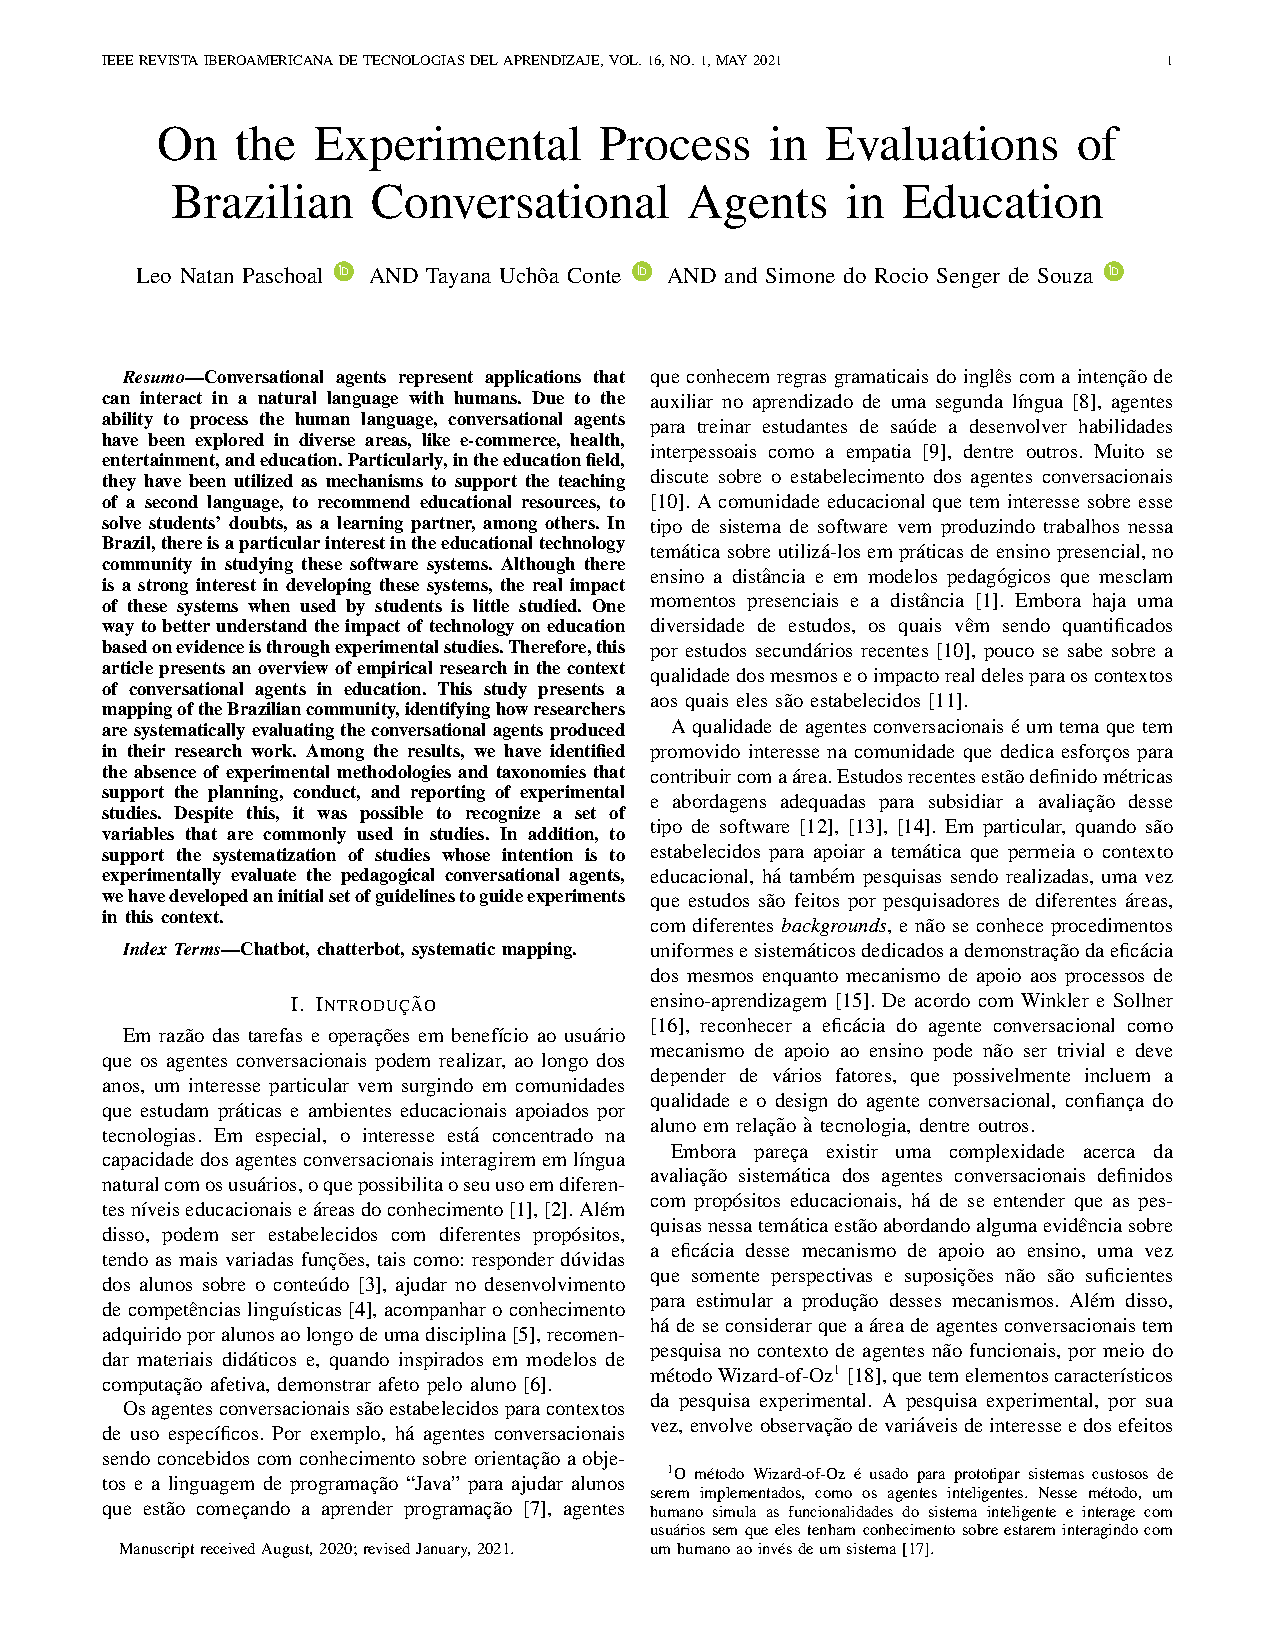
\includepdf[pages=-]{Textos_Quali/Coletanea/Mapeamento.pdf}

\chapter{Conversational Agent for Software Testing}\noindent Este capítulo é constituído pelo artigo intitulado ``Towards a Conversational Agent to Support the Software Testing Education'', de autoria principal de Leo Natan Paschoal, Lucas Fernandes Turci (colaborador no desenvolvimento do agente conversacional), Tayana Uchôa Conte e Simone do Rocio Senger de Souza (orientadoras do aluno). O artigo foi publicado no Simpósio Brasileiro de Engenharia de Software (qualis A3). Nele, os autores apresentam o desenvolvimento do agente conversacional como um mecanismo de apoio ao ensino de técnicas e critérios de teste de software. São discutidos aspectos considerados no seu desenvolvimento, a concepção das bases de conhecimento do agente e uma avaliação sobre a qualidade da interação fornecida pelo agente conversacional. Essa avaliação se baseou em um conjunto de métricas proposta por \citeonline{abushawar2016}. Ainda,  aspectos conceituais dos agentes conversacionais são abordados. Destaca-se que a versão incluída no capítulo segue o idioma adotado no projeto e o texto adere a estrutura utilizada pela conferência.
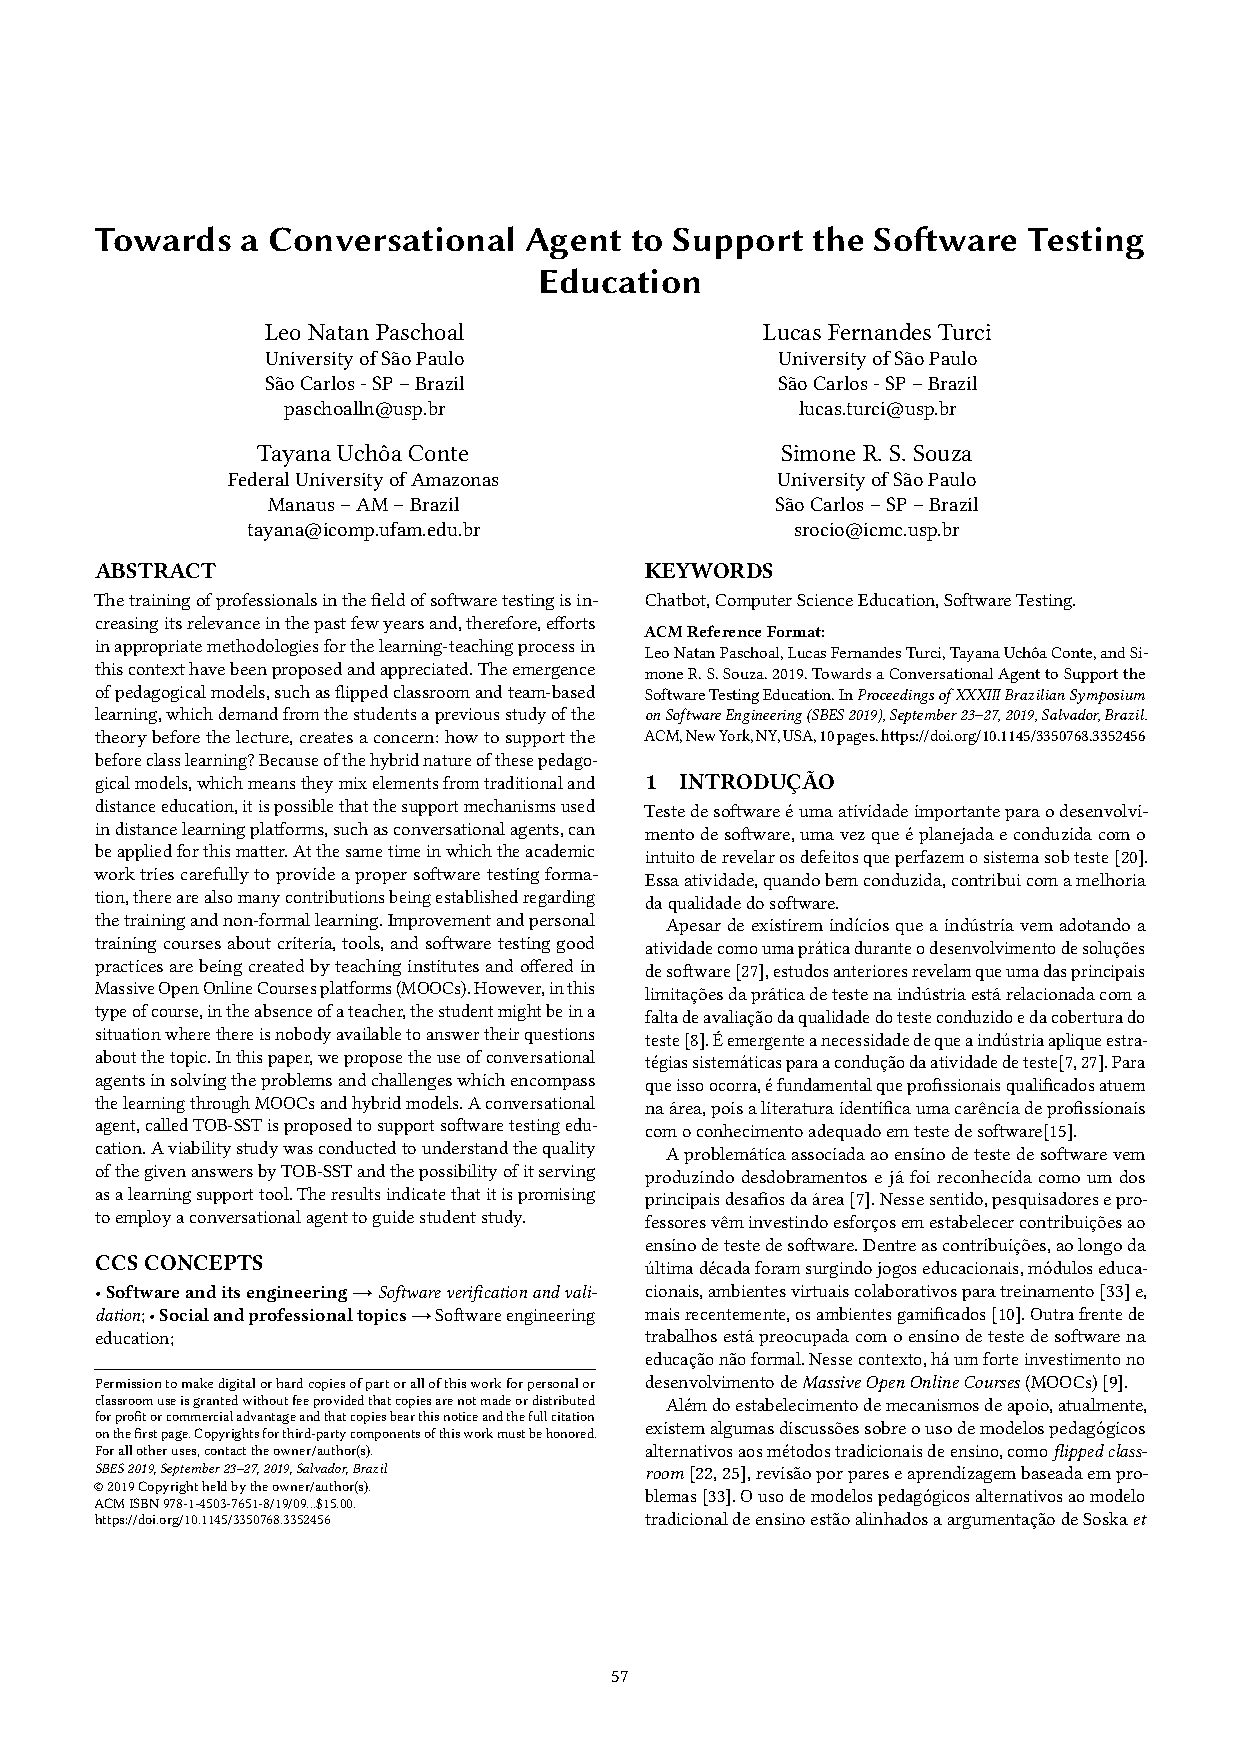
\includepdf[pages=-]{Textos_Quali/Coletanea/Tob.pdf}

\chapter{Conversational Agent in Software Testing Lessons}\noindent Este capítulo é constituído pelo artigo intitulado ``Evidences on the Educational Support offered by a Conversational Agent in Software Testing Lessons '', de autoria principal de Leo Natan Paschoal, Vânia de Oliveira Neves (colaboradora), Silvana Morita Melo (colaboradora),  Tayana Uchôa Conte e Simone do Rocio Senger de Souza (orientadoras do aluno). O artigo foi submetido para parecer e publicação no journal IEEE-RITA (qualis A3). Nele, os autores fazem um estudo experimental sobre a eficácia do apoio oferecido pelo agente conversacional TOB--STT em aulas de teste de software. No estudo, os autores consideraram o processo de \citeonline{Wohlin} e, ao final do estudo, compartilharam que problemas existem e que algumas ameaças à validade não foram mitigadas, passando a se tornar limitações associadas ao estudo. Os resultados do estudo oferecem discussões importantes que amparam e indicam a necessidade de novos estudos e evoluções no TOB--STT. Salienta-se que a versão incluída no capítulo acompanha o idioma adotado no projeto e o texto segue a estrutura do journal.
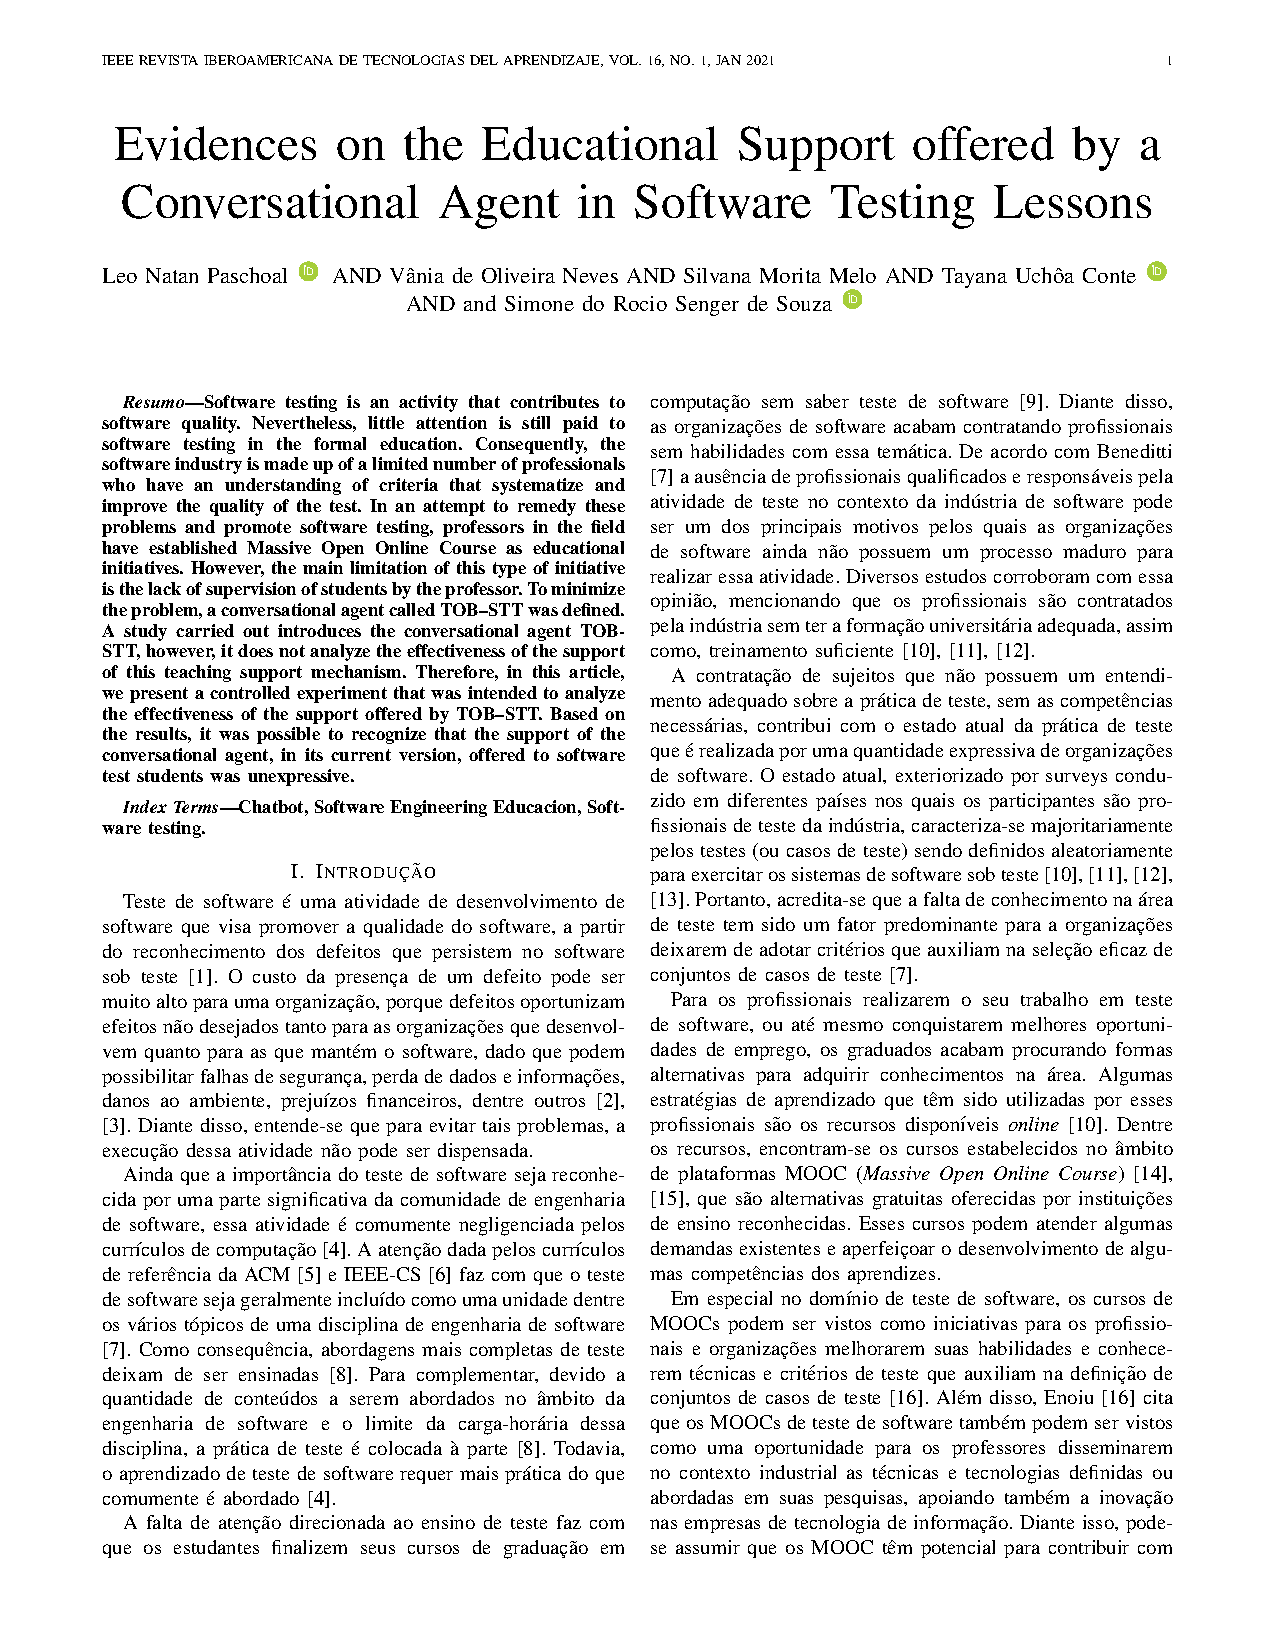
\includepdf[pages=-]{Textos_Quali/Coletanea/ExperimentoTob.pdf}

\chapter{Plano de Trabalho}
\label{chapter:config-pre-textual}
\noindent Este capítulo, constituído pela adaptação do material apresentado no Simpósio de Doutorado do XXIII Ibero-American Conference on Software Engineering\footnote{Versão original disponível em: $<$https://bit.ly/2OLqnwE$>$.}, apresenta os procedimentos que serão utilizados na condução do projeto de doutorado, as atividades que serão desenvolvidas, o cronograma de execução das atividades, assim como, os resultados e contribuições esperados ao término do projeto.


\section{Caracterização da pesquisa}

Sistemas conversacionais representam aplicações que são capazes de processar e emitir a linguagem humana, por meio de texto ou voz \cite{abdul2015survey}. Exemplos comuns dessas aplicações são os assistentes virtuais Siri\footnote{Mais informações disponíveis em $<$https://apple.co/2xjRw0X$>$.}, Google Assistant\footnote{Mais informações disponíveis em $<$http://bit.ly/39GniDQ$>$.} e Cortana\footnote{Mais informações disponíveis em $<$ http://bit.ly/2NnWZfA$>$.} \cite{Laranjo:2018}. Devido às habilidades do processamento de linguagem natural, essas aplicações têm sido estabelecidas para contextos de uso específicos, em diferentes áreas do conhecimento humano. Um dos maiores interesses para o uso desses sistemas é no domínio da educação. Isso pode ser observado em recentes estudos secundários que buscam definir um panorama sobre os sistemas conversacionais produzidos para fins educacionais \cite{hobert2019,io2017}. 

Por intermédio de estudos secundários, é possível observar que os sistemas conversacionais educacionais estão sendo produzidos para apoiar temáticas específicas, como o ensino de física, matemática, computação, engenharias, saúde, dentre outras. Além disso, eles são definidos com propósitos diferentes, na medida em que podem ser usados para solucionar dúvidas de alunos que não compreenderam um assunto, repassar informações que sejam relevantes, fornecer \textit{feedback} para as ações realizadas pelos estudantes, usar discurso motivacional para estimular os estudantes, contribuir com a aquisição de conhecimento do aluno, contribuir com o desenvolvimento de competências sociais, dentre outros. Ainda, eles podem ser definidos para se comportarem como tutores, companheiros de aprendizagem ou estudantes. 

A exploração do uso de sistemas conversacionais pedagógicos em cursos de plataformas \sigla{MOOCs}{\textit{Massive Open Online Courses}} tem se intensificado \cite{aguirre2018}, uma vez que esses cursos possuem uma ampla quantidade e diversidade de estudantes, e nem sempre há um professor disponível para atender aos questionamentos elaborados pelos alunos. Em trabalhos anteriores, o autor explorou o uso desses sistemas como apoio a práticas de ensino baseadas em metodologias ativas, como \textit{Flipped Classroom} \cite{Paschoal:2019}. Apesar de serem estimulados para uso em práticas ativas, esses sistemas também podem ser explorados no ensino tradicional (presencial ou a distância) \cite{krassmann2018}. Nesse sentido, podem ser usados em conjunto com outros recursos educacionais, tais como ambientes virtuais de aprendizagem, redes sociais, mundos virtuais e jogos educacionais.

Dado a versatilidade e aplicabilidade desses sistemas, era esperado que existissem mais estudos na literatura sobre a implantação dos mesmos em práticas educacionais. Todavia, observa-se que a comunidade não tem apresentado relatos sobre a implantação efetiva desses sistemas em cenários de ensino, pois a maioria dos trabalhos tem focado em descrever o desenvolvimento do sistema conversacional pedagógico e tem se distanciado em explorar sua implantação. Foram identificados estudos dedicados a avaliar, por exemplo, a usabilidade de sistemas conversacionais pedagógicos \cite{paschoal2018}. Também, foram encontrados estudos que descrevem o \textit{feedback} dos alunos ou do professor sobre o benefício do agente conversacional \cite{io2017,winkler2018}. No entanto, esses estudos são feitos pelos autores para comprovar alguma funcionalidade \cite{hobert2019}. Portanto, relatos de experiência da implantação dos sistemas conversacionais pedagógicos não são comuns em fóruns de divulgação científica.

Devido a falta de relatórios ou artigos científicos sobre as experiências em implantações desses sistemas, não existem registros de lições a serem aprendidas. Por outro lado, isso pode levar a alguns questionamentos associados à viabilidade das aplicações que estão sendo desenvolvidas. A viabilidade dos sistemas conversacionais poderia ser comprovada por meio de estudos experimentais, como é feito por pesquisadores de engenharia de software quando buscam compreender a viabilidade de técnicas, procedimentos e novas ferramentas \cite{Wohlin}. Trabalhos recentes apontam a falta de sistematização nos estudos que estão sendo produzidos no contexto de sistemas conversacionais \cite{winkler2018}. Sabe-se que isso dificulta o entendimento dos procedimentos e resultados apresentados e a sua replicação \cite{de2016experimentation}. Além disso, cada estudo avalia um aspecto do sistema conversacional, portanto, não há padronização no que é considerado durante a avaliação \cite{hobert2019}. Por exemplo, enquanto alguns pesquisadores avaliam somente aspectos técnicos dos sistemas conversacionais pedagógicos, outros consideram somente as percepções dos estudantes e não observam questões técnicas, como a qualidade da conversa. Desse modo, o entendimento que se tem é que que a comunidade da área ainda não apresenta de maneira clara os elementos que são importantes na avaliação de um sistema conversacional para o ensino.

Essa falta de pesquisas sobre avaliações no contexto de sistemas conversacionais pedagógicos pode ter relação com a falta de procedimentos de apoio à sistematização, como também a falta de conhecimento sobre a necessidade dessa sistematização \cite{io2017}. Como a área é constituída por pesquisadores com formações em diferentes domínios, é possível que as avaliações que estão sendo realizadas tenham relação direta com o que o pesquisador está acostumado a utilizar em trabalhos de sua área. Por exemplo, um pesquisador da área de engenharia pode não conhecer os procedimentos que apoiam a avaliação experimental utilizados por pesquisadores da área da computação.

Neste panorama e considerando que os sistemas conversacionais se diferem dos sistemas de software tradicionais, o desafio desta pesquisa de doutorado é ampliar a sistematização das avaliações sobre a viabilidade dos sistemas conversacionais pedagógicos e padronizar a avaliação conduzida por pesquisadores com diferentes \textit{backgrounds}. Assim, espera-se propor um framework de apoio para avaliações experimentais de sistemas conversacionais pedagógicos de modo que a viabilidade, qualidade e outros requisitos de interesse possam ser avaliados com maior confiabilidade. O objetivo é padronizar as avaliações experimentais de modo que os resultados possam ser melhor comparados. Busca-se promover direcionamentos para apoiar pesquisadores a definir avaliações sistemáticas de sistemas conversacionais pedagógicos, concentrando nos diferentes estágios de uma avaliação sistemática – a saber: planejamento, operação, execução e divulgação.

\section{Justificativa}

Os sistemas conversacionais emergem como sistemas de software com potencial para solucionar ou minimizar problemas associados ao ensino e a aprendizagem, uma vez que flexibilizam a interação entre usuário-computador e podem estar disponíveis para uso a todo momento, isto é, 24 horas por dia e 7 dias por semana \cite{Jain:2018}. Com base nessa premissa, muitos pesquisadores vêm tirando proveito desses sistemas para propor soluções às problemáticas que permeiam o âmbito educacional. No entanto, somente a proposta e o desenvolvimento desses sistemas não garante que os problemas estão sendo solucionados. 

De acordo com \citeonline{Shull} e  \citeonline{Travassos:2002}, os produtos de software não deveriam ser apenas propostos, desenvolvidos ou apresentados para venda sem experimentação e validação. Na visão de \citeonline{Basili:1998}, só é possível verificar se o entendimento atual sobre a temática está correto por meio de estudos experimentais. Desse modo, acredita-se que só é possível averiguar se sistemas conversacionais pedagógicos conseguem solucionar os problemas para os quais são propostos por meio da condução de estudos experimentais.

O paradigma experimental tem sido adotado e adaptado por diversas linhas de investigação dentro da Ciência da Computação, tais como Sistemas Operacionais \cite{FORTIER2003331} e Engenharia de Software \cite{Wohlin}. No âmbito da Engenharia de Software existem algumas definições para os propósitos da experimentação. \citeonline{Conradi:2001} descrevem que a experimentação auxilia a construir uma base de conhecimento confiável, permitindo reduzir as incertezas sobre quais as teorias, ferramentas e metodologias são adequadas. Adicionalmente, a experimentação elimina suposições errôneas e oferece suporte para orientar a teoria nas direções promissoras de pesquisa \cite{Conradi:2001}.

Apesar da experimentação estar bem estabelecida na área da engenharia de software, a condução de experimentos em outras áreas ainda não é uma prática habitual. De acordo com \citeonline{Kitchenham:2002}, algumas áreas de pesquisa têm dificuldade em realizar estudos experimentais. Em virtude disso, existem estudos que discutem sobre a necessidade de adaptar os modelos já estabelecidos e consolidados em outras áreas ou desenvolver modelos específicos para o domínio de investigação. Considerando as necessidades intrínsecas da área e tipos de aplicações, muitas áreas têm concentrado esforços para o estabelecimento de diretrizes, processos e \textit{frameworks} de apoio a experimentação. Em \citeonline{Vos:2012}, por exemplo, os autores apresentam um framework para pesquisa de experimental sobre técnicas e ferramentas de teste de software. Já na pesquisa de \citeonline{Sheard:2009}, por exemplo, os autores mencionam sobre a necessidade de adequação de um modelo de experimentação para ambientes de apoio ao ensino de programação. 

Em decorrência do atual estado da arte sobre os sistemas conversacionais pedagógicos, acredita-se que é necessário oferecer apoio metodológico, visando estimular a condução de estudos experimentais na área. Supõe-se que o apoio metodológico aumentará o rigor da pesquisa na área e contribuirá com a adesão de procedimentos sistemáticos durante a condução desses estudos. Adicionalmente, é necessário apoiar a replicação dos experimentos, estimulando a geração de pacotes de dados experimentais com conjunto de informações importantes para a replicação, buscando facilitar o compartilhamento e reúso de materiais produzidos, adotados e gerados durante a condução de experimentos.

\section{Solução proposta}

Considerando que o projeto de pesquisa conduzido no contexto do doutorado envolve a investigação e o estabelecimento de um framework para apoiar o planejamento, operação, condução e relato de estudos experimentais sobre sistemas conversacionais pedagógicos, busca-se:

\begin{enumerate}

   \item Estabelecer um vocabulário de experimentação para que pesquisadores conduzam e reportem seus estudos utilizando conceitos e terminologias comuns. O vocabulário é importante porque a comunidade de pesquisa que trabalha com sistemas conversacionais pedagógicos provêm de diferentes áreas do conhecimento humano e precisa conseguir utilizar a mesma linguagem para compartilhar os resultados de suas avaliações.

    \item Definir um corpo de conhecimento sobre variáveis e métricas. O corpo de conhecimento possibilitará ao usuário final do framework  reconhecer quais as variáveis que podem ser controladas e não podem ser controladas na condução de experimentos sobre sistemas conversacionais pedagógicos, dando ênfase a dois tipos de variáveis, a saber: variáveis dependentes e variáveis independentes. Nessa etapa, serão investigadas e classificadas as variáveis dependentes que são de interesse para estes sistemas (\textit{e.g.}, eficácia, desempenho, qualidade das respostas, qualidade da interface, funcionalidade, percepção e contribuição para o que se propõe). Adicionalmente, será definido, com base na literatura, um conjunto de possíveis métricas para essas variáveis.

   \item Produzir diretrizes para que os pesquisadores ao projetarem as avaliações experimentais possam identificar as possíveis ameças à validade do estudo. Essas diretrizes devem apresentar recomendações para evitá-las.

   \item Propor um guia de experimentação para a condução de experimentos sobre sistemas conversacionais pedagógicos. Nessa perspectiva, o guia indicará atividades que devem ser planejadas e realizadas durante a condução do experimento. O guia tem o propósito de orientar o usuário final do framework na realização das atividades para o planejamento e realização do experimento. Adicionalmente, o guia deverá indicar quais são as informações relevantes que devem compor o relatório do experimento.
   
   \item Desenvolver um agente conversacional com conhecimentos sobre experimentação. A intenção do agente será auxiliar o pesquisador a definir os procedimentos necessários para executar e reportar um estudo experimental sobre sistemas conversacionais educacionais. Portanto, o usuário poderá interagir em língua natural com o mecanismo de apoio e resolver suas dúvidas sobre o processo de experimentação.  
   
\end{enumerate}
 
Os artefatos descritos constituirão o framework metodológico, que também pode ser interpretado como um framework de pesquisa, cuja definição é baseada em \citeonline{Basili:1998} e consiste em uma estrutura organizacional que pode ser oferecida como uma meta genérica definida para ser instanciada em experimentos e em uma família de experimentos\footnote{Uma família de experimentos engloba um grupo de avaliações experimentais similares que estudam o mesmo objeto de estudo, considerando diferentes variações \cite{Basili:1998}.},  um conjunto de variáveis  para  ser explorado e usado no processo experimental, uma coleção de métricas para serem utilizadas como medidas às variáveis selecionadas no projeto experimental, etc. A Figura \ref{framework} apresenta uma ilustração de como o framework será constituído. Destaca-se o agente conversacional ao centro da figura, indicando que o modelo de conhecimento do agente conversacional contemplará o conhecimento sobre cada artefato.

\begin{figure}[!htb]
\centering
\caption{Uma visão geral do framework metodológico}
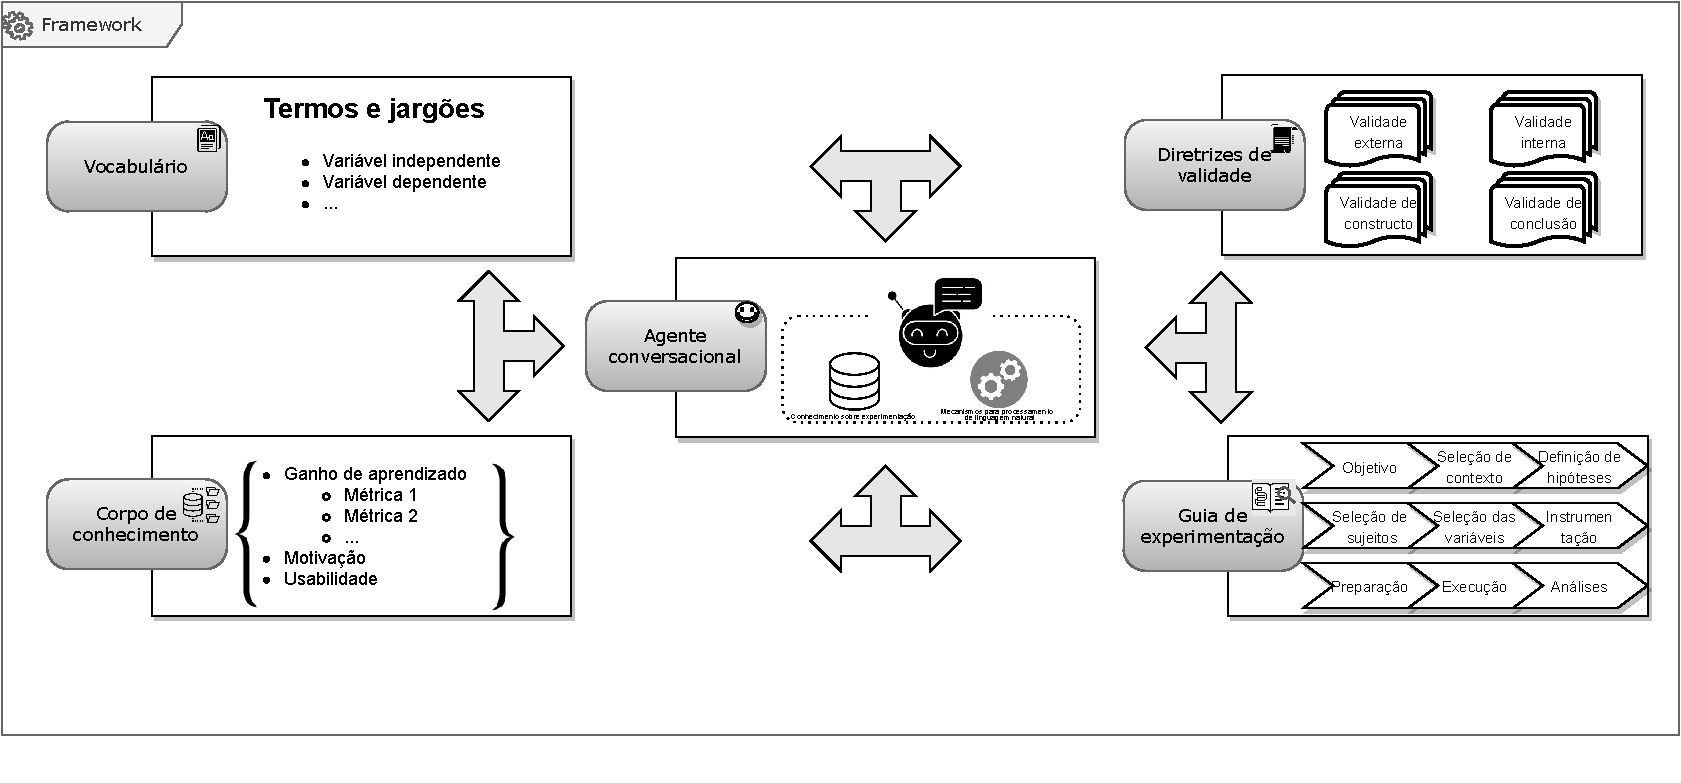
\includegraphics[width=0.95\textwidth]{Figuras/desenho.pdf}
\label{framework}
\fautor
\end{figure}
 
\section{Método de pesquisa} 

O framework metodológico proposto será constituído por um conjunto de artefatos. Dessa forma, a abordagem epistemológico-metodológica \textit{Design Science Research} será utilizada para caracterizar a pesquisa. Essa abordagem tem sido explorada em estudos que envolvem o estabelecimento de artefatos para um determinado contexto a fim de melhorar algo ou resolver um dado problema, especialmente em áreas como Engenharia de Software e Sistemas de Informação \cite{wieringa2014}. Os artefatos devem ser interpretados de forma ampla pela \textit{Design Science Research}, podendo ser constructos, algoritmos, métodos e frameworks.  

Um artefato é desenvolvido visando contribuir para melhor realização de um objetivo. Nesse sentido, a meta definida para este estudo, organizada no \textit{template} apresentado por \citeonline{wieringa2014}, consiste em: \underline{melhorar} os estudos experimentais sobre sistemas conversacionais educacionais, \underline{por meio de} um framework metodológico, \underline{que satisfaça} aspectos inerentes a validade de um experimento, replicação e generalização de resultados, \underline{para que} pesquisadores possam planejar, conduzir, executar e reportar de modo sistematizado os estudos experimentais. %Portanto, \underline{o artefato} discutido é o framework metodológico e \underline{o contexto} deste estudo é sistemas conversacionais educacionais.

Como envolve o desenvolvimento de um artefato (ou um conjunto de artefatos), espera-se que um ciclo de engenharia seja seguido. Para tanto, pode ser utilizado o ciclo de design apresentado em \citeonline{wieringa2014} ou o processo definido por \citeonline{Peffers:2007}. Neste estudo, será utilizado o processo definido por \citeonline{Peffers:2007}, que é composto por seis atividades. Vale salientar que a terminologia de cada atividade muda dependendo da base bibliográfica utilizada, mas as tarefas realizadas e a proposta principal são mantidas em cada interpretação do \textit{Design Science Research}. Em particular, as tarefas consideradas neste estudo são ilustradas pela Figura \ref{processoDSR}. Elas serão feitas, preferencialmente, seguindo um fluxo sequencial, com momentos de revisão e aprimoramento dos resultados.

\begin{figure}[!htb]
\centering
\caption{Processo de Design Science Research}
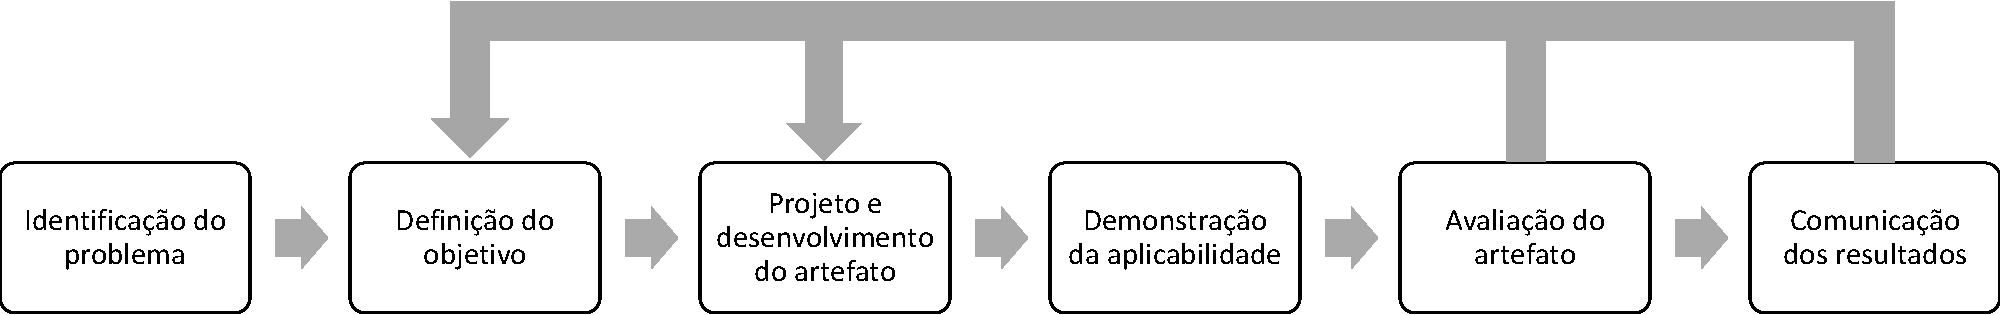
\includegraphics[width=0.95\textwidth]{Figuras/ProcessoDSR.pdf}
\label{processoDSR}
\fadaptada{Peffers:2007}
\end{figure}

Cada uma das atividades ilustradas na Figura \ref{processoDSR} é descrita a seguir:

 \begin{itemize}
    \item \textit{Identificação do problema:} a primeira tarefa envolve a investigação do problema, o reconhecimento das necessidades de uma temática e o valor de uma solução para esse problema;
    \item \textit{Definição do objetivo:} a segunda tarefa envolve a determinação do objetivo da pesquisa e identificação da viabilidade da solução proposta;
    \item \textit{Projeto e desenvolvimento do artefato:} a terceira tarefa envolve o estabelecimento propriamente dito do artefato, desde a especificações até a implementação;
    \item \textit{Demonstração da aplicabilidade:} a quarta tarefa envolve a demonstração da aplicação por meio de uma ou mais instanciações;
    \item \textit{Avaliação do artefato:} a quinta tarefa envolve a avaliação do artefato, considerando diferentes tipos de pesquisa (\textit{i.e.}, qualitativa ou quantitativa) e métodos (\textit{e.g.}, survey, estudo de caso, experimento controlado, dentre outros);  Salienta-se que a avaliação do artefato deve considerar os efeitos do artefato implementado. Portanto, pode englobar desdobramentos de pesquisas para compreender os efeitos gerados pelo artefato, até mesmo o entendimento sobre como o artefato causa tais efeitos;
    \item \textit{Comunicação dos resultados:} a sexta e última tarefa envolve o compartilhamento dos resultados alcançados para a comunidade de interesse, por meio de artigos científicos e relatórios técnicos.

 \end{itemize}
 
Como a pesquisa envolve vários artefatos que constituem o framework metodológico, a abordagem \textit{Design Science Research} será adotada em cada artefato e, portanto, no framework como um todo. A Tabela \ref{tab:atividades} descreve como cada tarefa do processo de \citeonline{Peffers:2007} está sendo utilizado na concepção do framework em sua totalidade. Apesar da adoção da abordagem, cada artefato será projetado e avaliado de formas distintas, considerando diferentes teorias para seu embasamento e métodos para avaliação. Por exemplo, um mapeamento sistemático da literatura pode ser utilizado para reforçar a necessidade de vocabulário, diretrizes para validade e um corpo de conhecimento de variáveis e métricas. 

\begin{table}[h]
\centering
\caption{Descrição das etapas de concepção do framework metodológico}
\begin{tabular}{p{5cm}p{10cm}}
\hline
\textbf{Atividade}                    & \textbf{Descrição}                                                                                                                                                                                                                                            \\ \hline
\multirow{4}{17em}{Identificação do problema}            & A identificação do problema aconteceu por meio de revisão bibliográfica, considerando principalmente estudos secundários realizados nos últimos anos sobre sistemas conversacionais educacionais                                                              \\
\multirow{4}{17em}{Definição do objetivo}                 & O objetivo foi definido no decorrer desta seção, considerando uma recomendação para descrição precisa de metas para pesquisas que utilizam a abordagem epistemológica \textit{Design Science Research}                                                              \\
\multirow{2}{17em}{Projeto e desenvolvimento} \multirow{3}{17em}{do artefato} & O projeto e desenvolvimento do artefato englobará a definição de cinco artefatos. Cada artefato será estabelecido de uma maneira, considerando suas diferentes características                                                                                \\
\multirow{2}{17em}{Demonstração da} \multirow{3}{17em}{aplicabilidade}        & Serão projetados exemplos com instancias do framework para sistemas conversacionais educacionais com diferentes requisitos e objetivos pedagógicos                                                                                                            \\
\multirow{5}{17em}{Avaliação do artefato}                 & O framework será avaliação por meio de um estudo experimental com pesquisadores que têm trabalhado com sistemas conversacionais pedagógicos, buscando reconhecer a completude e corretude dos designs de estudos experimentais projetados pelos pesquisadores \\
\multirow{2}{17em}{Comunicação dos resultados}            & Artigos científicos serão produzidos e apresentados em conferências e periódicos da temática                                                                                                                                                                  \\ \hline
\end{tabular}
\label{tab:atividades}

\end{table}

\section{Definição das atividades e cronograma}

Levando em consideração o método e objetivo descrito no decorrer da seção anterior, bem como a motivação e justificativas levantadas, apresenta-se, a seguir, as principais atividades a serem realizadas e que constituem o desenvolvimento deste projeto de doutorado:

\begin{itemize}

\item \textbf{Mapeamento das avaliações existentes:} inicialmente, serão localizados estudos que reportam a avaliação de sistemas conversacionais pedagógicos. Apesar desses não apresentarem avaliação sistemática, por meio deles é possível começar a identificar variáveis e métricas que poderão fazer parte do \textit{framework}. Para mapeá-los será replicado o mapeamento sistemático feito pelo autor e descrito em \citeonline{Paschoal:2020FIE}, incluindo critérios que permitem a seleção de estudos primários sobre sistemas conversacionais que abordem algum tipo de avaliação.

\item \textbf{Definição de um vocabulário:} a replicação do mapeamento permitirá ter um entendimento mais detalhado sobre o estado real de uso de conceitos e terminologias. Assim, considerando os estudos de \citeonline{Wohlin} e \citeonline{Shull}, será definido um vocabulário para experimentação de sistemas conversacionais pedagógicos. 

\item \textbf{Agrupamento de métodos e abordagens de avaliação:} um mapeamento sistemático sobre métodos e abordagens que são definidos para apoiar a avaliação de sistemas conversacionais está previsto. Espera-se que esse mapeamento possibilite a identificação de métricas, medidas e instrumentos que possam apoiar a definição do corpo de conhecimento sobre variáveis e métricas. 

\item \textbf{Construção do corpo de conhecimento:} Após a realização dos estudos secundários, as informações extraídas nos estudos selecionados devem ser reunidas, organizadas e disponibilizadas para acesso público como base de pesquisa e consulta. O corpo de conhecimento será definido considerando uma instanciação da abordagem de \citeonline{Vos:2012}.

\item \textbf{Reconhecimento e escrita das ameças à validade:} a definição das diretrizes para os pesquisadores reportarem ameaças à validade será inspirada em procedimentos adotados no estudo de \citeonline{de2016experimentation}. 

\item \textbf{Proposta de um guia de apoio à experimentação:} o guia para apoiar a experimentação de sistemas conversacionais pedagógicos será planejado considerando o processo experimental de \citeonline{Wohlin}. Esse guia ilustrará procedimentos e apresentará exemplos de planejamentos de experimentos.  

\item \textbf{Concepção do agente conversacional:} a concepção do agente conversacional levará em conta os artefatos estabelecidos ao longo da pesquisa para modelar o conhecimento do agente. Além disso, as experiências do autor no desenvolvimento desse tipo de software, que foram compartilhadas em estudos anteriores \cite{Paschoal:2019, paschoal2018}, serão utilizadas.

\item \textbf{Avaliação do framework:} após a definição dos artefatos, o \textit{framework} de pesquisa proposto será avaliado. A avaliação será realizado por meio de um estudo experimental conduzido com pesquisadores que trabalham com sistemas conversacionais pedagógicos.

\item \textbf{Condução de experimentos no contexto do TOB--STT: } ao passo que o framework seja construído, almeja-se utilizar os artefatos para projetar e conduzir estudos experimentais com a intenção de aprimorar o agente TOB--STT e compreender o seu impacto no ensino de teste de software.

\end{itemize}


Além disso, de acordo com as exigências do Programa de Pós-Graduação em Ciências de Computação e Matemática Computacional (CCMC), para obtenção do título de Doutor, outras atividades são obrigatórias, a saber:

\begin{itemize}

\item \textbf{Obtenção dos créditos para o curso de doutorado:} de acordo com o regulamento vigente do Programa de Pós-Graduação em Ciências da Computação e Matemática Computacional, alunos regulares no curso de doutorado devem cumprir pelo menos 44 créditos em disciplinas oferecidas pelo programa para o depósito da dissertação. Atualmente, o aluno cumpriu 45 créditos, obtendo conceito A em todas as disciplinas. A Tabela \ref{tab:creditos} apresenta algumas informações sobre as disciplinas cursadas.

\begin{table}[h]
\centering
\caption{Obtenção de créditos em disciplinas}
\label{tab:creditos}
\begin{tabular}{p{7cm}ccc}
\hline
\textbf{Disciplina} & \textbf{Carga horária} & \textbf{Créditos} & \textbf{Conceito} \\ \hline
Fundamentos do Gerenciamento Ágil de Projetos & 180 & 12 & A \\
Validação e Teste de Software & 180 & 12 & A \\
Interação Usuário-Computador I: Fundamentos & 120 & 8 & A \\
Interação Usuário-Computador II: Prática & 60 & 4 & A \\
Empreendedorismo & 90 & 6 & A \\
Atividades de Cultura e Extensão Universitária na Pós-Graduação & 30 & 2 & A \\
Tópicos em Computação e Matemática Computacional II & 15 & 1 & A \\ \hline
\end{tabular}
\end{table}

\item \textbf{Exame de proficiência em língua estrangeira:} no prazo de 18 meses do início do curso de doutorado é exigido ao aluno a comprovação de proficiência na língua inglesa, considerando pontuação e exames definidos pelo programa em conjunto com a Pró-reitora de Pós-graduação. O aluno comprovou proficiência no primeiro mês do curso, cumprindo esse requisito.

\item \textbf{Redação da monografia de qualificação e defesa no exame de qualificação:} de acordo com o regimento do programa, todo aluno deve passar por um exame de qualificação, a ser realizado em até 18 meses após o início do curso. Para tanto, o aluno redigiu esta monografia e apresentará até maio de 2021 a uma banca composta por três professores doutores, presidiada pelas orientadoras do estudante.

\item \textbf{Elaboração de artigos científicos:} os resultados obtidos ao longo do estudo devem ser organizados e escritos em formato de artigos científicos. Conforme o regimento do programa, são esperados artigos publicados em conferências nacionais e internacionais e em journal de relevância para a linha de pesquisa do programa. Ao menos, a coordenação do programa exige a publicação de um journal.

\item \textbf{Redação da tese e defesa do doutorado:} ao final dos 48 meses de matriculado do aluno, o aluno deve depositar e apresentar a tese, redigita em português ou inglês, que conterá os resultados de pesquisa obtidos ao longo do período. A defesa deverá ser feito em idioma equivalente ao texto redigido, em uma banca constituída por três professores doutores.

\end{itemize}

O cronograma apresentado no Quadro \ref{tab:schedule} especifica a atividade e o período em que a mesma será realizada.

%\onehalfspace

\newcommand{\y}{\rule{13,5pt}{5pt}}
\newcommand{\x}{\hspace*{5pt}}
\setlength{\tabcolsep}{0pt}
\begin{quadro}[!ht] 
\footnotesize
\caption{Cronograma}
\begin{tabular}{|l|c|c|c|c|c|c|c|c|c|c|c|c|c|c|c|c|}
  \cline{2-17}
  \multicolumn{1}{l|}{} & \multicolumn{3}{c|}{2019} & \multicolumn{4}{c|}{2020}  & \multicolumn{4}{c|}{2021} & \multicolumn{4}{c|}{2022}& \multicolumn{1}{c|}{2023}\\
  \cline{2-17}
  \multicolumn{1}{c|}{\textbf{Atividades}} &
  \rotatebox{90}{Abr-Jun\hspace{2pt}} &
  \rotatebox{90}{Jul-Set\hspace{2pt}} &
  \rotatebox{90}{Out-Dez\hspace{2pt}} &
  \rotatebox{90}{Jan-Mar\hspace{2pt}} &
  \rotatebox{90}{Abr-Jun\hspace{2pt}} &
  \rotatebox{90}{Jul-Set\hspace{2pt}} &
  \rotatebox{90}{Out-Dez\hspace{2pt}} &
  \rotatebox{90}{Jan-Mar\hspace{2pt}} &
  \rotatebox{90}{Abr-Jun\hspace{2pt}} &
  \rotatebox{90}{Jul-Set\hspace{2pt}} &
  \rotatebox{90}{Out-Dez\hspace{2pt}} &
  \rotatebox{90}{Jan-Mar\hspace{2pt}} &
  \rotatebox{90}{Abr-Jun\hspace{2pt}} &
  \rotatebox{90}{Jul-Set\hspace{2pt}} &
  \rotatebox{90}{Out-Dez\hspace{2pt}} &
  \rotatebox{90}{Jan-Mar\hspace{2pt}} 
  %\rotatebox{90}{Nov-Dec\hspace{2pt}} &
  %\rotatebox{90}{Jan-Feb\hspace{2pt}} &
  %\rotatebox{90}{Mar-Apr\hspace{2pt}} &
  %\rotatebox{90}{May-Jun\hspace{2pt}} &
  %\rotatebox{90}{Jul-Aug\hspace{2pt}} &
  %\rotatebox{90}{Sep-Oct\hspace{2pt}} &
  %\rotatebox{90}{Nov-Dec\hspace{2pt}} &
  %\rotatebox{90}{Jan-Feb\hspace{2pt}} 
  \\
  \hline
  Mapeamento das avaliações        
  & \x & \x & \x & \y & \x & \x & \x & \y & \y & \x & \x & \x & \x & \x & \x & \x  \\
  \hline
  Vocabulário           
  & \x & \x & \x & \x & \x & \x & \x & \x & \y & \y & \x & \x & \x & \x & \x & \x  \\
  \hline
  Agrupamento de métodos e abordagens  
  & \x & \x & \x & \x & \x & \x & \x & \x & \x & \x & \y & \x & \x & \x & \x & \x  \\
  \hline
  Corpo de conhecimento
  & \x & \x & \x & \x & \x & \x & \x & \x & \x & \x & \y & \x & \x & \x & \x & \x  \\
  \hline
  Escrita das ameaças
  & \x & \x & \x & \x & \x & \x & \x & \x & \x & \x & \x & \y & \x & \x & \x & \x  \\
  \hline
  Guia de experimentação
  & \x & \x & \x & \x & \x & \x & \x & \x & \x & \x & \x & \x & \y & \x & \x & \x  \\
  \hline
  Agente conversacional
  & \x & \x & \x & \x & \x & \x & \x & \x & \x & \x & \x & \x & \x & \y & \x & \x  \\
  \hline
  Avaliação do framework
  & \x & \x & \x & \x & \x & \x & \x & \x & \x & \x & \x & \x & \x & \x & \y & \x  \\
  \hline
  Experimentos no TOB--STT
  & \x & \x & \y & \x & \x & \y & \x & \x & \x & \y & \x & \x & \y & \x & \y & \y  \\
  \hline  
  Créditos do curso          
  & \y & \y & \y & \x & \x & \x & \x & \x & \x & \x & \x & \x & \x & \x & \x & \x  \\
  \hline
  Proficiência  
  & \y & \x & \x & \x & \x & \x & \x & \x & \x & \x & \x & \x & \x & \x & \x & \x  \\
  \hline
  Qualificação          
  & \x & \x & \x & \x & \x & \x & \y & \y & \x & \x & \x & \x & \x & \x & \x & \x  \\
  \hline
  Artigos
  & \x & \x & \y & \x & \y & \y & \x & \x & \y & \x & \y & \x & \y & \x & \x & \y  \\
  \hline
  Tese          
  & \x & \x & \x & \x & \x & \x & \x & \y & \x & \x & \x & \x & \x & \x & \x & \y  \\
  \hline
\end{tabular}
 \label{tab:schedule}
\end{quadro}


\section{Resultados esperados}

Com o desenvolvimento deste projeto de doutorado espera-se obter as seguintes contribuições:

\begin{enumerate}

\item Aprofundar os estudos sobre avaliações no contexto de sistemas conversacionais educacionais.

\item Fortalecer o entendimento que a comunidade vinculada aos sistemas conversacionais educacionais tem sobre avaliações sistemáticas.

\item Aprimorar a condução de estudos experimentais por intermédio de um corpo de conhecimento e um guia de experimentação.

\item Possibilitar o desenvolvimento de sistemas conversacionais com mais qualidade, uma vez que a partir dos estudos experimentais é possível analisar adequadamente a viabilidade das soluções propostas.

\item Ampliar a credibilidade dos sistemas conversacionais como mecanismo de apoio ao ensino.

\item Consolidar o agente conversacional TOB--STT como um mecanismo eficaz de apoio ao ensino de teste de software.

\item Auxiliar na formação de recursos humanos em Engenharia de Software considerando desenvolver um projeto de iniciação científica atrelado ao projeto em questão e desdobramento de novos projetos de mestrado e doutorado.

\end{enumerate}




% ---
% Finaliza a parte no bookmark do PDF, para que se inicie o bookmark na raiz
% ---
\bookmarksetup{startatroot}% 
% ---

% ----------------------------------------------------------
% ELEMENTOS PÓS-TEXTUAIS
% ----------------------------------------------------------
\postextual

% ----------------------------------------------------------
% Referências bibliográficas
% ----------------------------------------------------------
\bibliography{references}

% ---------------------------------------------------------------------
% GLOSSÁRIO
% ---------------------------------------------------------------------

% ----------------------------------------------------------
% Apêndices
% ---------------------------------------------------------

% ----------------------------------------------------------
% Anexos
% ----------------------------------------------------------

% ---
\end{document}